\subsection{Amplificatore differenziale}

\begin{wrapfigure}[14]{l}{0.5\textwidth}
  \begin{center}
    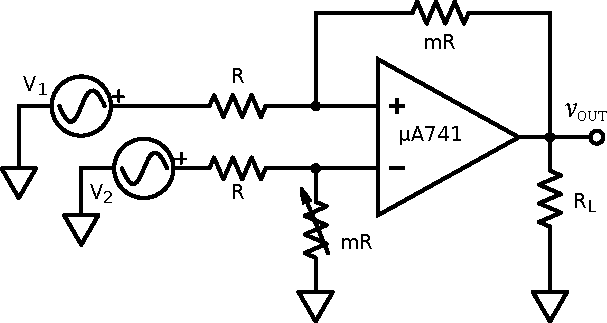
\includegraphics[width=0.280\textwidth]{../E05/latex/c_teo_diff_amp.pdf}
  \end{center}
  \caption{...}
  \label{cir5:diff_amp_teo}
\end{wrapfigure}

In questa parte dell'esperienza cercheremo di capire e analizzare un amplificatore differenziale (\ref{cir5:diff_amp}). Oltre al fatto che scegliendo i valori di resistenza possiamo decidere il guadagno, la proprietà più importante è sicuramente il vantaggio che si ha rispetto al rumore in modo comune. Per capirne il motivo analizziamo il circuito riportato in figura (\ref{cir5:diff_amp_teo}).

Sfruttiamo il principio di sovrapposizione per valutare la tensione in uscita in funzione delle due di ingresso. Ricordiamo che la sovrapposizione può essere applicata per sistemi lineari. Ciò è molto utile in quanto ci permette di separare l'analisi circuitale e ricondurci a casi più semplici.

Chiamiamo $V_-$ la tensione all'ingresso invertente e $V_+$ quella all'ingresso non invertente. Poniamo $V_1=0$. La tensione le punto $V_+$ sarà ovviamente data dal partitore con $R$ ed $mR$. Assumendo l'op-amp ideale, abbiamo $V_+=V_-$. Possiamo dunque scrivere:

\begin{equation}
\begin{cases} V_+=V_-  \\ V_+=V_2\frac{mR}{R+mR} \\ V_-= V_{out2}\frac{R}{R+mR}\end{cases}  \Rightarrow V_{out2}=mV_2
\label{eq 5: vout2}
\end{equation}

\begin{wrapfigure}[13]{r}{0.5\textwidth}
  \begin{center}
    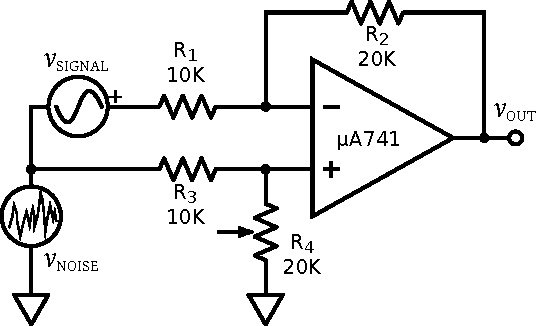
\includegraphics[width=0.280\textwidth]{../E05/latex/c_diff_amp.pdf}
  \end{center}
  \caption{...}
  \label{cir5:diff_amp}
\end{wrapfigure}

Analogamente, poniamo $V_2=0$. Otteniamo le seguenti equazioni del circuito:

\begin{equation}
\begin{cases} V_+=V_-=0  \\ \frac{V_1}{R}+\frac{V_{out2}}{mR}=0 \end{cases}  \Rightarrow V_{out1}=-mV_1
\label{eq 5: vout1}
\end{equation}

Sommando ora (\ref{eq 5: vout2}) e (\ref{eq 5: vout2}) otteniamo trivialmente $V_{out}=m(V_2-V_1)$.

Possiamo ora passare ad analizzare il circuito da cui siamo partiti, ovvero quello affetto da noise riportato in figura (\ref{cir5:diff_amp}). Possiamo scrivere, senza perdere di generalità,
$$
\begin{cases} V_1=V_{in}+V_{noise} \\ V_2=V_{noise} \end{cases}  \Rightarrow V_{out}=m(V_{noise}-(V_{in}+V_{noise}))=-V_{in}
$$

L'amplificatore differenziale ci permette dunque di eliminare in modo efficace il rumore di modo comune. 

Come vediamo, la resistenza collegata tra comune e $V_+$ è in realtà un trimmer. Ciò è necessario in quanto, non essendo esattamente uguali le resistenze ed essendo reale l'op-amp, prima di utilizzare il circuito è necessario bilanciare il circuito in modo da ottenere un segnale il più piccolo possibile quando i segnali in ingresso sono uguali. 

Il laboratorio abbiamo utilizzato come sorgente di noise il generatore di forme d'onda e come $V_{in}$ il generatore di tensione costante. Abbiamo utilizzato delle R da \SI{10}{\kilo\ohm} e $mR=2R$. La resistenza variabile è stata costruita mettendo in serie una da \SI{10}{\kilo\ohm} con un trimmer sempre da \SI{10}{\kilo\ohm}. Per controllare il bilanciamento abbiamo connesso entrambi gli ingressi al generatore di forme d'onda ed è stato utilizzato un segnale sinusoidale di $20Vpp$. Il segnale in uscita è stato dunque riportato sull'oscilloscopio. Abbiamo notato che cambiando il valore della resistenza con il trimmer il segnale in uscita cambiava. Il miglior bilanciamento che siamo riusciti a raggiungere a portato la tensione picco-picco del rumore a \SI{0.5}{\milli\volt}. Abbiamo dunque riattaccato il generatore di tensione costante e alimentato il circuito con $2Vpp$. Il rumore è sempre stato simulato con una sinusoidale di $20Vpp$. I risultati sono riportati nella seguente figura.

$$GRAFICO$$

Come vediamo, il rumore è stato completamente eliminato dall'amplificatore differenziale. Abbiamo successivamente provato a sbilanciare il circuito, per vedere l'effetto del rumore sul segnale in uscita. E' stato dunque variata la resistenza con trimmer e abbiamo utilizzato un rumore con dei picchi molto accentuati, così da vedere bene gli effetti sul segnale in uscita. 

$$GRAFICO$$

Come vediamo, il segnale risulta disturbato dal rumore. Inoltre, il guadagno può essere cambiato solo se si cambiano 2 resistenze nel circuito. Una soluzione efficace che inoltre rimedia alla bassa impedenza in ingresso è quella di utilizzare un Amplificatore per Strumentazione.